\documentclass[12pt,a4paper]{article}

\usepackage[a4paper,text={16.5cm,25.2cm},centering, margin=1in]{geometry}

\usepackage[scale=0.95]{FiraMono}
\usepackage[utf8]{inputenc}
\usepackage[T1]{fontenc}
\usepackage{mathpazo}

\usepackage{amssymb,amsmath}
\usepackage{bm}
\usepackage{graphicx}
\usepackage{microtype}
\usepackage{hyperref}
\setlength{\parindent}{0pt}
\setlength{\parskip}{1.2ex}

\usepackage{fvextra}
\DefineVerbatimEnvironment{Highlighting}{Verbatim}{breaklines,commandchars=\\\{\}}

\setcounter{secnumdepth}{0}

\hypersetup
       {   pdfauthor = { Akanksha Srivastava (as2752) },
           pdftitle={ BEE 4750/5750 Homework 3 },
           colorlinks=TRUE,
           linkcolor=black,
           citecolor=blue,
           urlcolor=blue
       }

\title{ BEE 4750/5750 Homework 3 }

\author{ Akanksha Srivastava (as2752) }

\date{ 2022-10-14 }

\usepackage{upquote}
\usepackage{listings}
\usepackage{xcolor}
\lstset{
    basicstyle=\ttfamily\footnotesize,
    upquote=true,
    breaklines=true,
    breakindent=0pt,
    keepspaces=true,
    showspaces=false,
    columns=fullflexible,
    showtabs=false,
    showstringspaces=false,
    escapeinside={(*@}{@*)},
    extendedchars=true,
}
\newcommand{\HLJLt}[1]{#1}
\newcommand{\HLJLw}[1]{#1}
\newcommand{\HLJLe}[1]{#1}
\newcommand{\HLJLeB}[1]{#1}
\newcommand{\HLJLo}[1]{#1}
\newcommand{\HLJLk}[1]{\textcolor[RGB]{148,91,176}{\textbf{#1}}}
\newcommand{\HLJLkc}[1]{\textcolor[RGB]{59,151,46}{\textit{#1}}}
\newcommand{\HLJLkd}[1]{\textcolor[RGB]{214,102,97}{\textit{#1}}}
\newcommand{\HLJLkn}[1]{\textcolor[RGB]{148,91,176}{\textbf{#1}}}
\newcommand{\HLJLkp}[1]{\textcolor[RGB]{148,91,176}{\textbf{#1}}}
\newcommand{\HLJLkr}[1]{\textcolor[RGB]{148,91,176}{\textbf{#1}}}
\newcommand{\HLJLkt}[1]{\textcolor[RGB]{148,91,176}{\textbf{#1}}}
\newcommand{\HLJLn}[1]{#1}
\newcommand{\HLJLna}[1]{#1}
\newcommand{\HLJLnb}[1]{#1}
\newcommand{\HLJLnbp}[1]{#1}
\newcommand{\HLJLnc}[1]{#1}
\newcommand{\HLJLncB}[1]{#1}
\newcommand{\HLJLnd}[1]{\textcolor[RGB]{214,102,97}{#1}}
\newcommand{\HLJLne}[1]{#1}
\newcommand{\HLJLneB}[1]{#1}
\newcommand{\HLJLnf}[1]{\textcolor[RGB]{66,102,213}{#1}}
\newcommand{\HLJLnfm}[1]{\textcolor[RGB]{66,102,213}{#1}}
\newcommand{\HLJLnp}[1]{#1}
\newcommand{\HLJLnl}[1]{#1}
\newcommand{\HLJLnn}[1]{#1}
\newcommand{\HLJLno}[1]{#1}
\newcommand{\HLJLnt}[1]{#1}
\newcommand{\HLJLnv}[1]{#1}
\newcommand{\HLJLnvc}[1]{#1}
\newcommand{\HLJLnvg}[1]{#1}
\newcommand{\HLJLnvi}[1]{#1}
\newcommand{\HLJLnvm}[1]{#1}
\newcommand{\HLJLl}[1]{#1}
\newcommand{\HLJLld}[1]{\textcolor[RGB]{148,91,176}{\textit{#1}}}
\newcommand{\HLJLs}[1]{\textcolor[RGB]{201,61,57}{#1}}
\newcommand{\HLJLsa}[1]{\textcolor[RGB]{201,61,57}{#1}}
\newcommand{\HLJLsb}[1]{\textcolor[RGB]{201,61,57}{#1}}
\newcommand{\HLJLsc}[1]{\textcolor[RGB]{201,61,57}{#1}}
\newcommand{\HLJLsd}[1]{\textcolor[RGB]{201,61,57}{#1}}
\newcommand{\HLJLsdB}[1]{\textcolor[RGB]{201,61,57}{#1}}
\newcommand{\HLJLsdC}[1]{\textcolor[RGB]{201,61,57}{#1}}
\newcommand{\HLJLse}[1]{\textcolor[RGB]{59,151,46}{#1}}
\newcommand{\HLJLsh}[1]{\textcolor[RGB]{201,61,57}{#1}}
\newcommand{\HLJLsi}[1]{#1}
\newcommand{\HLJLso}[1]{\textcolor[RGB]{201,61,57}{#1}}
\newcommand{\HLJLsr}[1]{\textcolor[RGB]{201,61,57}{#1}}
\newcommand{\HLJLss}[1]{\textcolor[RGB]{201,61,57}{#1}}
\newcommand{\HLJLssB}[1]{\textcolor[RGB]{201,61,57}{#1}}
\newcommand{\HLJLnB}[1]{\textcolor[RGB]{59,151,46}{#1}}
\newcommand{\HLJLnbB}[1]{\textcolor[RGB]{59,151,46}{#1}}
\newcommand{\HLJLnfB}[1]{\textcolor[RGB]{59,151,46}{#1}}
\newcommand{\HLJLnh}[1]{\textcolor[RGB]{59,151,46}{#1}}
\newcommand{\HLJLni}[1]{\textcolor[RGB]{59,151,46}{#1}}
\newcommand{\HLJLnil}[1]{\textcolor[RGB]{59,151,46}{#1}}
\newcommand{\HLJLnoB}[1]{\textcolor[RGB]{59,151,46}{#1}}
\newcommand{\HLJLoB}[1]{\textcolor[RGB]{102,102,102}{\textbf{#1}}}
\newcommand{\HLJLow}[1]{\textcolor[RGB]{102,102,102}{\textbf{#1}}}
\newcommand{\HLJLp}[1]{#1}
\newcommand{\HLJLc}[1]{\textcolor[RGB]{153,153,119}{\textit{#1}}}
\newcommand{\HLJLch}[1]{\textcolor[RGB]{153,153,119}{\textit{#1}}}
\newcommand{\HLJLcm}[1]{\textcolor[RGB]{153,153,119}{\textit{#1}}}
\newcommand{\HLJLcp}[1]{\textcolor[RGB]{153,153,119}{\textit{#1}}}
\newcommand{\HLJLcpB}[1]{\textcolor[RGB]{153,153,119}{\textit{#1}}}
\newcommand{\HLJLcs}[1]{\textcolor[RGB]{153,153,119}{\textit{#1}}}
\newcommand{\HLJLcsB}[1]{\textcolor[RGB]{153,153,119}{\textit{#1}}}
\newcommand{\HLJLg}[1]{#1}
\newcommand{\HLJLgd}[1]{#1}
\newcommand{\HLJLge}[1]{#1}
\newcommand{\HLJLgeB}[1]{#1}
\newcommand{\HLJLgh}[1]{#1}
\newcommand{\HLJLgi}[1]{#1}
\newcommand{\HLJLgo}[1]{#1}
\newcommand{\HLJLgp}[1]{#1}
\newcommand{\HLJLgs}[1]{#1}
\newcommand{\HLJLgsB}[1]{#1}
\newcommand{\HLJLgt}[1]{#1}


\begin{document}

\maketitle

%  This setups the environment and installs packages, but doesn't appear in the generated document 
%  You shouldn't need to modify this 


% - this block is hidden, but stores the generator and demand data; you can use a dataframe to combine these or refactor as you'd like 


\section{Problem 1}
\subsection{Problem 1.1}
For this problem, the decision variables are: 

\begin{itemize}
\item[1. ] The installed capacity (MW) of generator type g: $x_g$


\item[2. ] The production (MW) from generator type g in period t: $y_{g,t}$


\item[3. ] The nonserved load (MW) in each period t: $nse_t$

\end{itemize}
Here, generators types include geothermal, coal, CCGT, CT, wind, and solar. Periods include every hour from 1 to 24.

We can begin to implement our model in Julia:


\begin{lstlisting}
(*@\HLJLnB{julia>}@*) (*@\HLJLk{using}@*) (*@\HLJLn{JuMP}@*)

(*@\HLJLnB{julia>}@*) (*@\HLJLk{using}@*) (*@\HLJLn{HiGHS}@*)

(*@\HLJLnB{julia>}@*) (*@\HLJLn{gencap}@*) (*@\HLJLoB{=}@*) (*@\HLJLnf{Model}@*)(*@\HLJLp{(}@*)(*@\HLJLn{HiGHS}@*)(*@\HLJLoB{.}@*)(*@\HLJLn{Optimizer}@*)(*@\HLJLp{);}@*)

(*@\HLJLnB{julia>}@*) (*@\HLJLn{generators}@*) (*@\HLJLoB{=}@*) (*@\HLJLp{[}@*)(*@\HLJLs{"{}geo"{}}@*)(*@\HLJLp{,}@*)(*@\HLJLs{"{}coal"{}}@*)(*@\HLJLp{,}@*)(*@\HLJLs{"{}ccgt"{}}@*)(*@\HLJLp{,}@*)(*@\HLJLs{"{}ct"{}}@*)(*@\HLJLp{,}@*)(*@\HLJLs{"{}wind"{}}@*)(*@\HLJLp{,}@*)(*@\HLJLs{"{}solar"{}}@*)(*@\HLJLp{];}@*)

(*@\HLJLnB{julia>}@*) (*@\HLJLn{G}@*) (*@\HLJLoB{=}@*) (*@\HLJLni{1}@*)(*@\HLJLoB{:}@*)(*@\HLJLnf{length}@*)(*@\HLJLp{(}@*)(*@\HLJLn{generators}@*)(*@\HLJLp{);}@*)

(*@\HLJLnB{julia>}@*) (*@\HLJLn{T}@*) (*@\HLJLoB{=}@*) (*@\HLJLni{1}@*)(*@\HLJLoB{:}@*)(*@\HLJLnf{length}@*)(*@\HLJLp{(}@*)(*@\HLJLn{hours}@*)(*@\HLJLp{);}@*)

(*@\HLJLnB{julia>}@*) (*@\HLJLnd{@variable}@*)(*@\HLJLp{(}@*)(*@\HLJLn{gencap}@*)(*@\HLJLp{,}@*)(*@\HLJLn{x}@*)(*@\HLJLp{[}@*)(*@\HLJLn{G}@*)(*@\HLJLp{]}@*)(*@\HLJLoB{>=}@*)(*@\HLJLni{0}@*)(*@\HLJLp{);}@*)

(*@\HLJLnB{julia>}@*) (*@\HLJLnd{@variable}@*)(*@\HLJLp{(}@*)(*@\HLJLn{gencap}@*)(*@\HLJLp{,}@*)(*@\HLJLn{y}@*)(*@\HLJLp{[}@*)(*@\HLJLn{G}@*)(*@\HLJLp{,}@*)(*@\HLJLn{T}@*)(*@\HLJLp{]}@*)(*@\HLJLoB{>=}@*)(*@\HLJLni{0}@*)(*@\HLJLp{);}@*)

(*@\HLJLnB{julia>}@*) (*@\HLJLnd{@variable}@*)(*@\HLJLp{(}@*)(*@\HLJLn{gencap}@*)(*@\HLJLp{,}@*)(*@\HLJLn{ns}@*)(*@\HLJLp{[}@*)(*@\HLJLn{T}@*)(*@\HLJLp{]}@*)(*@\HLJLoB{>=}@*)(*@\HLJLni{0}@*)(*@\HLJLp{)}@*);
\end{lstlisting}

\subsection{Problem 1.2}
The objective function is to minimize the total cost of generation, which is the sum of the investment cost and the operating cost.  If $C_g^{INV}$ is the investment cost for generator g, $C_g^{OP}$ is the operating cost for generator g, and $L_t$ is the length  of time period $t$:

\[
minZ = \sum_g C_g^{INV}x_g + \sum_g\sum_t L_t C_g^{OP} y_{g,t} + \sum_t NSE_{cost} nse_t
\]
In Julia, this becomes:


\begin{lstlisting}
(*@\HLJLnB{julia>}@*) (*@\HLJLnd{@objective}@*)(*@\HLJLp{(}@*)(*@\HLJLn{gencap}@*)(*@\HLJLp{,}@*)(*@\HLJLn{Min}@*)(*@\HLJLp{,}@*)(*@\HLJLn{investment{\_}cost}@*)(*@\HLJLoB{{\textquotesingle}*}@*)(*@\HLJLn{x}@*) (*@\HLJLoB{+}@*) (*@\HLJLni{365}@*)(*@\HLJLoB{*}@*)(*@\HLJLp{(}@*)(*@\HLJLni{22}@*)(*@\HLJLoB{*}@*)(*@\HLJLnf{sum}@*)(*@\HLJLp{(}@*)(*@\HLJLn{y}@*)(*@\HLJLp{[}@*)(*@\HLJLni{2}@*)(*@\HLJLp{,}@*)(*@\HLJLoB{:}@*)(*@\HLJLp{])}@*) (*@\HLJLoB{+}@*) (*@\HLJLni{35}@*)(*@\HLJLoB{*}@*)(*@\HLJLnf{sum}@*)(*@\HLJLp{(}@*)(*@\HLJLn{y}@*)(*@\HLJLp{[}@*)(*@\HLJLni{3}@*)(*@\HLJLp{,}@*)(*@\HLJLoB{:}@*)(*@\HLJLp{])}@*) (*@\HLJLoB{+}@*) (*@\HLJLni{45}@*)(*@\HLJLoB{*}@*)(*@\HLJLnf{sum}@*)(*@\HLJLp{(}@*)(*@\HLJLn{y}@*)(*@\HLJLp{[}@*)(*@\HLJLni{4}@*)(*@\HLJLp{,}@*)(*@\HLJLoB{:}@*)(*@\HLJLp{])}@*) (*@\HLJLoB{+}@*) (*@\HLJLni{1000}@*)(*@\HLJLoB{*}@*)(*@\HLJLnf{sum}@*)(*@\HLJLp{(}@*)(*@\HLJLn{ns}@*)(*@\HLJLp{)))}@*);
\end{lstlisting}

\subsection{Problem 1.3}
Derive all relevant constraints (you don\ensuremath{\rq}t need to write them all out, but they should all be represented through your notation).  Make sure to include any needed justifications or derivations. Why is your set of constraints complete?

The constraints of this problem include installed capacity and availability, the need to serve the load  in all time frames, and nonnegativity. These can be written out as follows:

\begin{itemize}
\item[1. ] Installed Capacity and Availability: In a given time period, our $y_{g,t}$ cannot exceed the installed capacity multiplied by the capacity factor, as it is not possibly for the generator to produce more than that quantity. When $CF_g$ is the capacity factor for a given generator,

\end{itemize}
\[
y_{g,t}\ensuremath{\leq}CF_g*x_g
\]
\begin{itemize}
\item[2. ] Serving Load: The sum of the generated electricity and the nonserved load should equal the demand for that time period, $D_t$.

\end{itemize}
\[
\sum_{g} y_{g,t} + nse_t = D_t
\]
\begin{itemize}
\item[3. ] Nonnegativity: Our installed capacities, productions, and nonserved loads cannot be negative (this is physically not possible). 

\end{itemize}
\[
x_g \ensuremath{\geq} 0, y_{g,t} \ensuremath{\geq} 0, nse_t \ensuremath{\geq} 0
\]
.

In Julia, this translates to:


\begin{lstlisting}
(*@\HLJLnB{julia>}@*) (*@\HLJLcs{{\#}}@*) (*@\HLJLcs{Availability}@*) (*@\HLJLcs{Constraints}@*)
       (*@\HLJLn{avail}@*) (*@\HLJLoB{=}@*) (*@\HLJLnf{zeros}@*)(*@\HLJLp{(}@*)(*@\HLJLnf{length}@*)(*@\HLJLp{(}@*)(*@\HLJLn{G}@*)(*@\HLJLp{),}@*)(*@\HLJLnf{length}@*)(*@\HLJLp{(}@*)(*@\HLJLn{T}@*)(*@\HLJLp{));}@*)

(*@\HLJLnB{julia>}@*) (*@\HLJLn{avail}@*)(*@\HLJLp{[}@*)(*@\HLJLni{1}@*)(*@\HLJLp{,}@*)(*@\HLJLoB{:}@*)(*@\HLJLp{]}@*) (*@\HLJLoB{=}@*) (*@\HLJLn{thermal{\_}cf}@*)(*@\HLJLp{[}@*)(*@\HLJLni{1}@*)(*@\HLJLp{]}@*)(*@\HLJLoB{*}@*)(*@\HLJLnf{ones}@*)(*@\HLJLp{(}@*)(*@\HLJLnf{length}@*)(*@\HLJLp{(}@*)(*@\HLJLn{T}@*)(*@\HLJLp{));}@*)

(*@\HLJLnB{julia>}@*) (*@\HLJLn{avail}@*)(*@\HLJLp{[}@*)(*@\HLJLni{2}@*)(*@\HLJLoB{:}@*)(*@\HLJLni{4}@*)(*@\HLJLp{,}@*)(*@\HLJLoB{:}@*)(*@\HLJLp{]}@*) (*@\HLJLoB{=}@*) (*@\HLJLn{thermal{\_}cf}@*)(*@\HLJLp{[}@*)(*@\HLJLni{2}@*)(*@\HLJLoB{:}@*)(*@\HLJLni{4}@*)(*@\HLJLp{]}@*)(*@\HLJLoB{*}@*)(*@\HLJLnf{ones}@*)(*@\HLJLp{(}@*)(*@\HLJLnf{length}@*)(*@\HLJLp{(}@*)(*@\HLJLn{T}@*)(*@\HLJLp{))}@*)(*@\HLJLoB{{\textquotesingle}}@*)(*@\HLJLp{;}@*)

(*@\HLJLnB{julia>}@*) (*@\HLJLn{avail}@*)(*@\HLJLp{[}@*)(*@\HLJLni{5}@*)(*@\HLJLp{,}@*)(*@\HLJLoB{:}@*)(*@\HLJLp{]}@*) (*@\HLJLoB{=}@*) (*@\HLJLn{wind{\_}cf}@*)(*@\HLJLp{;}@*)

(*@\HLJLnB{julia>}@*) (*@\HLJLn{avail}@*)(*@\HLJLp{[}@*)(*@\HLJLni{6}@*)(*@\HLJLp{,}@*)(*@\HLJLoB{:}@*)(*@\HLJLp{]}@*) (*@\HLJLoB{=}@*) (*@\HLJLn{solar{\_}cf}@*)(*@\HLJLp{;}@*)

(*@\HLJLnB{julia>}@*) (*@\HLJLnd{@constraint}@*)(*@\HLJLp{(}@*)(*@\HLJLn{gencap}@*)(*@\HLJLp{,}@*)(*@\HLJLn{availability}@*)(*@\HLJLp{[}@*)(*@\HLJLn{g}@*) (*@\HLJLkp{in}@*) (*@\HLJLn{G}@*)(*@\HLJLp{,}@*) (*@\HLJLn{t}@*) (*@\HLJLkp{in}@*) (*@\HLJLn{T}@*)(*@\HLJLp{],}@*) (*@\HLJLn{y}@*)(*@\HLJLp{[}@*)(*@\HLJLn{g}@*)(*@\HLJLp{,}@*)(*@\HLJLn{t}@*)(*@\HLJLp{]}@*) (*@\HLJLoB{<=}@*) (*@\HLJLn{avail}@*)(*@\HLJLp{[}@*)(*@\HLJLn{g}@*)(*@\HLJLp{,}@*)(*@\HLJLn{t}@*)(*@\HLJLp{]}@*)(*@\HLJLoB{*}@*)(*@\HLJLn{x}@*)(*@\HLJLp{[}@*)(*@\HLJLn{g}@*)(*@\HLJLp{]);}@*)

(*@\HLJLnB{julia>}@*) (*@\HLJLcs{{\#}}@*) (*@\HLJLcs{Load}@*) (*@\HLJLcs{Constraints}@*)
       (*@\HLJLnd{@constraint}@*)(*@\HLJLp{(}@*)(*@\HLJLn{gencap}@*)(*@\HLJLp{,}@*)(*@\HLJLn{load}@*)(*@\HLJLp{[}@*)(*@\HLJLn{t}@*) (*@\HLJLkp{in}@*) (*@\HLJLn{T}@*)(*@\HLJLp{],}@*) (*@\HLJLnf{sum}@*)(*@\HLJLp{(}@*)(*@\HLJLn{y}@*)(*@\HLJLp{[}@*)(*@\HLJLoB{:}@*)(*@\HLJLp{,}@*)(*@\HLJLn{t}@*)(*@\HLJLp{])}@*) (*@\HLJLoB{+}@*) (*@\HLJLn{ns}@*)(*@\HLJLp{[}@*)(*@\HLJLn{t}@*)(*@\HLJLp{]}@*) (*@\HLJLoB{==}@*) (*@\HLJLn{demand}@*)(*@\HLJLp{[}@*)(*@\HLJLn{t}@*)(*@\HLJLp{])}@*);
\end{lstlisting}

\subsection{Problem 1.4}

\begin{lstlisting}
(*@\HLJLnB{julia>}@*) (*@\HLJLnf{optimize!}@*)(*@\HLJLp{(}@*)(*@\HLJLn{gencap}@*)(*@\HLJLp{)}@*)
Presolving model
156 rows, 162 cols, 420 nonzeros
156 rows, 162 cols, 420 nonzeros
Presolve : Reductions: rows 156(-12); columns 162(-12); elements 420(-24)
Solving the presolved LP
Using EKK dual simplex solver - serial
  Iteration        Objective     Infeasibilities num(sum)
          0     0.0000000000e+00 Pr: 24(60321.5) 0s
        120     9.1214221224e+08 Pr: 0(0) 0s
Solving the original LP from the solution after postsolve
Model   status      : Optimal
Simplex   iterations: 120
Objective value     :  9.1214221224e+08
HiGHS run time      :          0.00
\end{lstlisting}

\subsection{Problem 1.5}
Answering the relevant questions using the following block of code:


\begin{lstlisting}
(*@\HLJLnB{julia>}@*) (*@\HLJLcs{{\#}}@*) (*@\HLJLcs{Installed}@*) (*@\HLJLcs{Capacity}@*) (*@\HLJLcs{for}@*) (*@\HLJLcs{Each}@*) (*@\HLJLcs{Generating}@*) (*@\HLJLcs{Plant}@*)
       (*@\HLJLn{installed{\_}capacity}@*) (*@\HLJLoB{=}@*) (*@\HLJLn{value}@*)(*@\HLJLoB{.}@*)(*@\HLJLp{(}@*)(*@\HLJLn{x}@*)(*@\HLJLp{);}@*)

(*@\HLJLnB{julia>}@*) (*@\HLJLcs{{\#}}@*) (*@\HLJLcs{Total}@*) (*@\HLJLcs{Cost}@*)
       (*@\HLJLn{total{\_}cost}@*) (*@\HLJLoB{=}@*) (*@\HLJLnf{objective{\_}value}@*)(*@\HLJLp{(}@*)(*@\HLJLn{gencap}@*)(*@\HLJLp{);}@*)

(*@\HLJLnB{julia>}@*) (*@\HLJLcs{{\#}}@*) (*@\HLJLcs{Nonserved}@*) (*@\HLJLcs{Energy}@*)
       (*@\HLJLn{nonserved{\_}energy{\_}total}@*) (*@\HLJLoB{=}@*) (*@\HLJLnf{sum}@*)(*@\HLJLp{(}@*)(*@\HLJLn{value}@*)(*@\HLJLoB{.}@*)(*@\HLJLp{(}@*)(*@\HLJLn{ns}@*)(*@\HLJLp{))}@*);
\end{lstlisting}

Therefore we get that the installed capacities for geothermal, coal, CCGT, CT, wind and solar are 0 MW, 0 MW, 1704 MW, 881 MW, 1238 MW, and 2729 MW respectively. The total cost for the expansion in this case would be  912,142,212 dollars, and the nonserved load would be 0 MW.

\subsection{Problem 1.6}

\begin{lstlisting}
(*@\HLJLnB{julia>}@*) (*@\HLJLcs{{\#}}@*) (*@\HLJLcs{Assign}@*) (*@\HLJLcs{generations}@*) (*@\HLJLcs{to}@*) (*@\HLJLcs{generator}@*) (*@\HLJLcs{type}@*)
       (*@\HLJLn{served{\_}load}@*) (*@\HLJLoB{=}@*) (*@\HLJLnf{ones}@*)(*@\HLJLp{(}@*)(*@\HLJLnf{length}@*)(*@\HLJLp{(}@*)(*@\HLJLn{G}@*)(*@\HLJLp{),}@*)(*@\HLJLnf{length}@*)(*@\HLJLp{(}@*)(*@\HLJLn{T}@*)(*@\HLJLp{));}@*) (*@\HLJLn{served{\_}load}@*)(*@\HLJLp{[}@*)(*@\HLJLoB{:}@*)(*@\HLJLp{,}@*)(*@\HLJLoB{:}@*)(*@\HLJLp{]}@*)(*@\HLJLoB{=}@*)(*@\HLJLn{value}@*)(*@\HLJLoB{.}@*)(*@\HLJLp{(}@*)(*@\HLJLn{y}@*)(*@\HLJLp{)[}@*)(*@\HLJLoB{:}@*)(*@\HLJLp{,}@*)(*@\HLJLoB{:}@*)(*@\HLJLp{];}@*)

(*@\HLJLnB{julia>}@*) (*@\HLJLk{using}@*) (*@\HLJLn{Plots}@*)

(*@\HLJLnB{julia>}@*) (*@\HLJLcs{{\#}}@*) (*@\HLJLcs{Plotting}@*) (*@\HLJLcs{Line}@*) (*@\HLJLcs{Plots}@*) (*@\HLJLcs{for}@*) (*@\HLJLcs{Raw}@*) (*@\HLJLcs{Amounts}@*)
       (*@\HLJLnf{plot}@*)(*@\HLJLp{(}@*)(*@\HLJLn{hours}@*)(*@\HLJLp{,}@*)(*@\HLJLn{served{\_}load}@*)(*@\HLJLp{[}@*)(*@\HLJLni{1}@*)(*@\HLJLp{,}@*)(*@\HLJLoB{:}@*)(*@\HLJLp{],}@*)(*@\HLJLn{label}@*)(*@\HLJLoB{=}@*)(*@\HLJLs{"{}Geo"{}}@*)(*@\HLJLp{,}@*)(*@\HLJLn{xlabel}@*)(*@\HLJLoB{=}@*)(*@\HLJLs{"{}Hour"{}}@*)(*@\HLJLp{,}@*)(*@\HLJLn{ylabel}@*)(*@\HLJLoB{=}@*)(*@\HLJLs{"{}Generation}@*) (*@\HLJLs{(MW)"{}}@*)(*@\HLJLp{,}@*)(*@\HLJLn{title}@*)(*@\HLJLoB{=}@*)(*@\HLJLs{"{}Energy}@*) (*@\HLJLs{Generation}@*) (*@\HLJLs{vs}@*) (*@\HLJLs{Time"{}}@*)(*@\HLJLp{);}@*)

(*@\HLJLnB{julia>}@*) (*@\HLJLnf{plot!}@*)(*@\HLJLp{(}@*)(*@\HLJLn{hours}@*)(*@\HLJLp{,}@*)(*@\HLJLn{served{\_}load}@*)(*@\HLJLp{[}@*)(*@\HLJLni{2}@*)(*@\HLJLp{,}@*)(*@\HLJLoB{:}@*)(*@\HLJLp{],}@*)(*@\HLJLn{label}@*)(*@\HLJLoB{=}@*)(*@\HLJLs{"{}Coal"{}}@*)(*@\HLJLp{);}@*)

(*@\HLJLnB{julia>}@*) (*@\HLJLnf{plot!}@*)(*@\HLJLp{(}@*)(*@\HLJLn{hours}@*)(*@\HLJLp{,}@*)(*@\HLJLn{served{\_}load}@*)(*@\HLJLp{[}@*)(*@\HLJLni{3}@*)(*@\HLJLp{,}@*)(*@\HLJLoB{:}@*)(*@\HLJLp{],}@*)(*@\HLJLn{label}@*)(*@\HLJLoB{=}@*)(*@\HLJLs{"{}CCGT"{}}@*)(*@\HLJLp{);}@*)

(*@\HLJLnB{julia>}@*) (*@\HLJLnf{plot!}@*)(*@\HLJLp{(}@*)(*@\HLJLn{hours}@*)(*@\HLJLp{,}@*)(*@\HLJLn{served{\_}load}@*)(*@\HLJLp{[}@*)(*@\HLJLni{4}@*)(*@\HLJLp{,}@*)(*@\HLJLoB{:}@*)(*@\HLJLp{],}@*)(*@\HLJLn{label}@*)(*@\HLJLoB{=}@*)(*@\HLJLs{"{}CT"{}}@*)(*@\HLJLp{);}@*)

(*@\HLJLnB{julia>}@*) (*@\HLJLnf{plot!}@*)(*@\HLJLp{(}@*)(*@\HLJLn{hours}@*)(*@\HLJLp{,}@*)(*@\HLJLn{served{\_}load}@*)(*@\HLJLp{[}@*)(*@\HLJLni{5}@*)(*@\HLJLp{,}@*)(*@\HLJLoB{:}@*)(*@\HLJLp{],}@*)(*@\HLJLn{label}@*)(*@\HLJLoB{=}@*)(*@\HLJLs{"{}Wind"{}}@*)(*@\HLJLp{);}@*)

(*@\HLJLnB{julia>}@*) (*@\HLJLnf{plot!}@*)(*@\HLJLp{(}@*)(*@\HLJLn{hours}@*)(*@\HLJLp{,}@*)(*@\HLJLn{served{\_}load}@*)(*@\HLJLp{[}@*)(*@\HLJLni{6}@*)(*@\HLJLp{,}@*)(*@\HLJLoB{:}@*)(*@\HLJLp{],}@*)(*@\HLJLn{label}@*)(*@\HLJLoB{=}@*)(*@\HLJLs{"{}Solar"{}}@*))
\end{lstlisting}
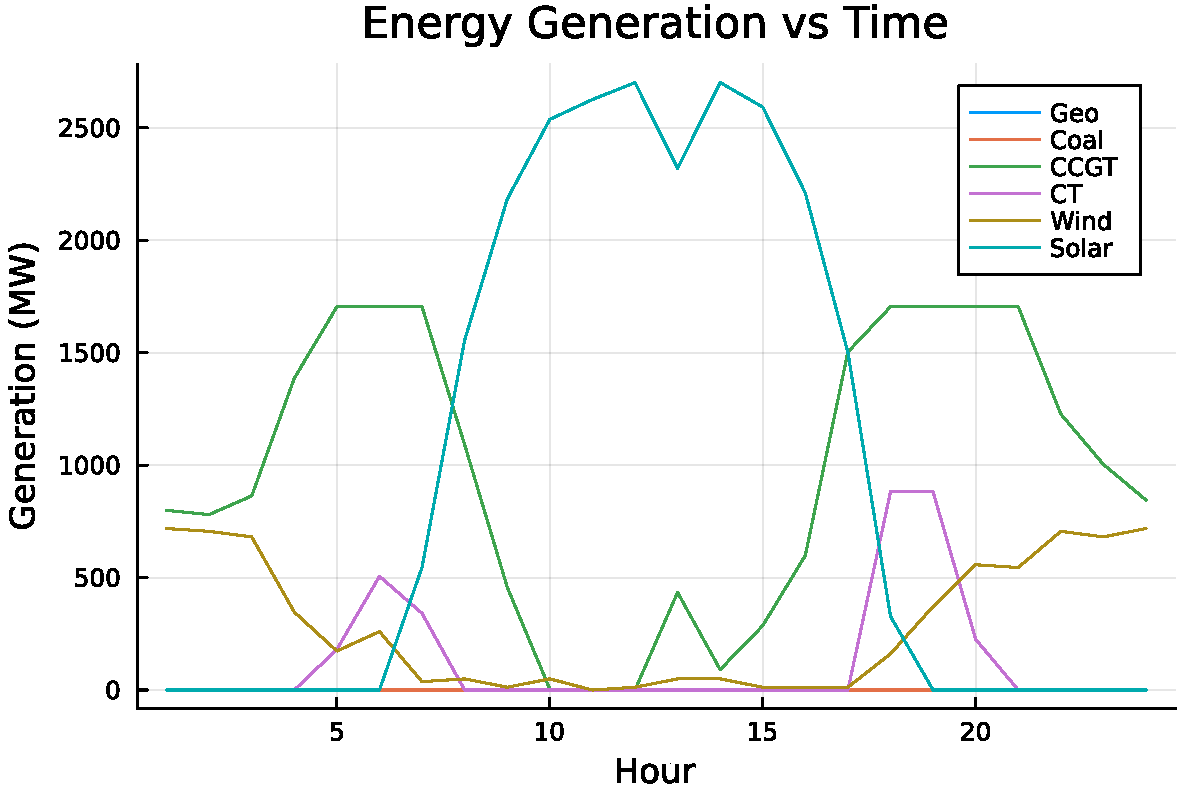
\includegraphics[width=\linewidth]{figures/as2752_hw3_8_1.pdf}

\begin{lstlisting}
(*@\HLJLnB{julia>}@*) (*@\HLJLcs{{\#}}@*) (*@\HLJLcs{Plotting}@*) (*@\HLJLcs{Area}@*) (*@\HLJLcs{Plot}@*) (*@\HLJLcs{for}@*) (*@\HLJLcs{Overall}@*) (*@\HLJLcs{Contributions}@*)
       (*@\HLJLnf{areaplot}@*)(*@\HLJLp{(}@*)(*@\HLJLn{hours}@*)(*@\HLJLp{,}@*)(*@\HLJLn{served{\_}load}@*)(*@\HLJLoB{{\textquotesingle}}@*)(*@\HLJLp{,}@*)(*@\HLJLn{label}@*)(*@\HLJLoB{=}@*)(*@\HLJLnf{permutedims}@*)(*@\HLJLp{([}@*)(*@\HLJLs{"{}Geo"{}}@*)(*@\HLJLp{,}@*)(*@\HLJLs{"{}Coal"{}}@*)(*@\HLJLp{,}@*)(*@\HLJLs{"{}CCGT"{}}@*)(*@\HLJLp{,}@*)(*@\HLJLs{"{}CT"{}}@*)(*@\HLJLp{,}@*)(*@\HLJLs{"{}Wind"{}}@*)(*@\HLJLp{,}@*)(*@\HLJLs{"{}Solar"{}}@*)(*@\HLJLp{]),}@*)(*@\HLJLn{xlabel}@*)(*@\HLJLoB{=}@*)(*@\HLJLs{"{}Hour"{}}@*)(*@\HLJLp{,}@*)(*@\HLJLn{ylabel}@*)(*@\HLJLoB{=}@*)(*@\HLJLs{"{}Generation"{}}@*)(*@\HLJLp{,}@*)(*@\HLJLn{title}@*)(*@\HLJLoB{=}@*)(*@\HLJLs{"{}Stacked}@*) (*@\HLJLs{Energy}@*) (*@\HLJLs{Generation}@*) (*@\HLJLs{vs}@*) (*@\HLJLs{Time"{}}@*))
\end{lstlisting}
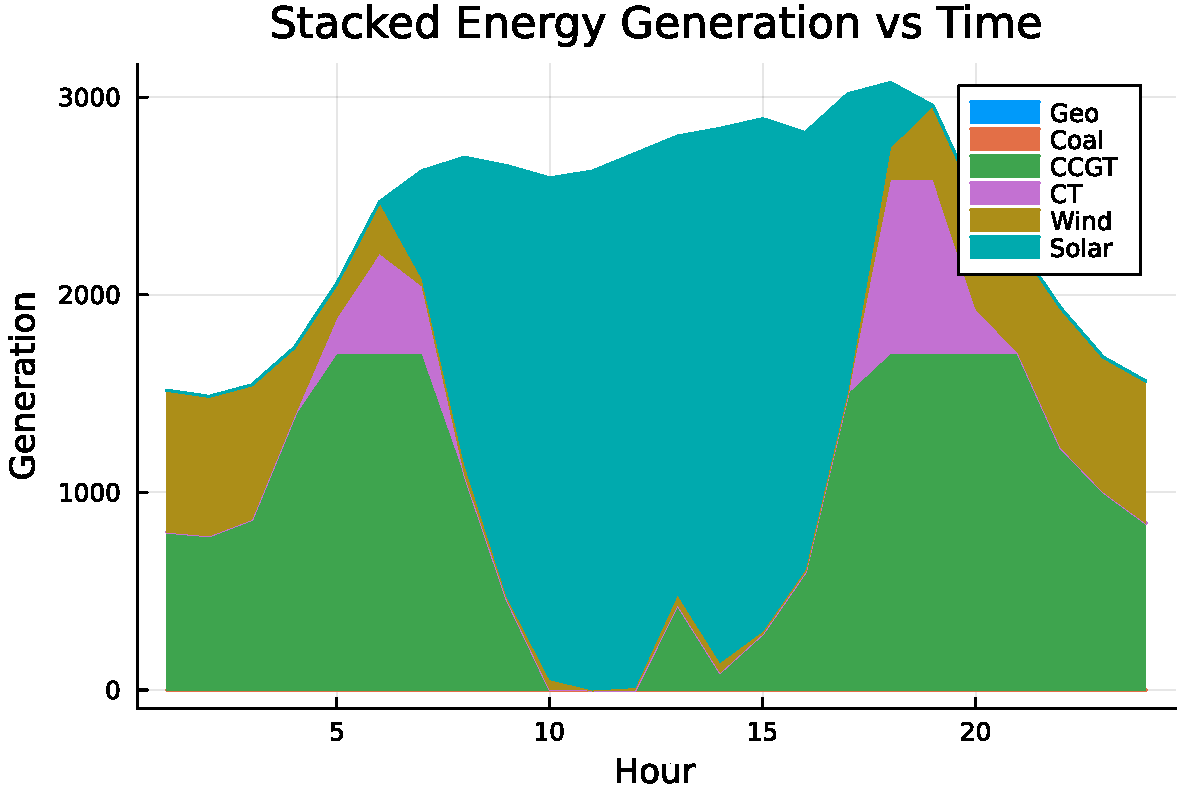
\includegraphics[width=\linewidth]{figures/as2752_hw3_8_2.pdf}

\section{Problem 2}
\subsection{Problem 2.1}
\subsection{Problem 2.2}
\subsection{Problem 2.3}
\subsection{Problem 2.4}
\subsection{Problem 2.5}
\section{References}


\end{document}